\chapter{Projective Geometry}

\section{The Projective Space}

\section{Fundamental Theorem of Projective Geometry}

\section{Some Theorems}

\begin{theorem}[Desargues's Theorem]
\end{theorem}

\begin{proof}
  Consider the figure
  \begin{figure}[H]
   \center
   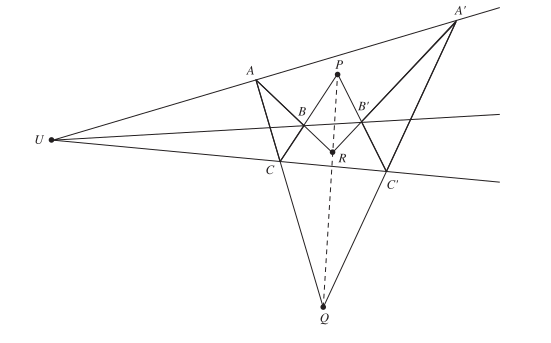
\includegraphics[width=0.85\linewidth]{desargues.png}
   \caption{Figure from \cite{brannan}.}
  \end{figure}
\end{proof}

\begin{remark}
  Proof adapted from \cite{brannan}, with some modifications.
\end{remark}

\begin{theorem}[Pascal's Theorem]

\end{theorem}

\begin{proof}
  Consider the figure
  \begin{figure}[H]
   \center
   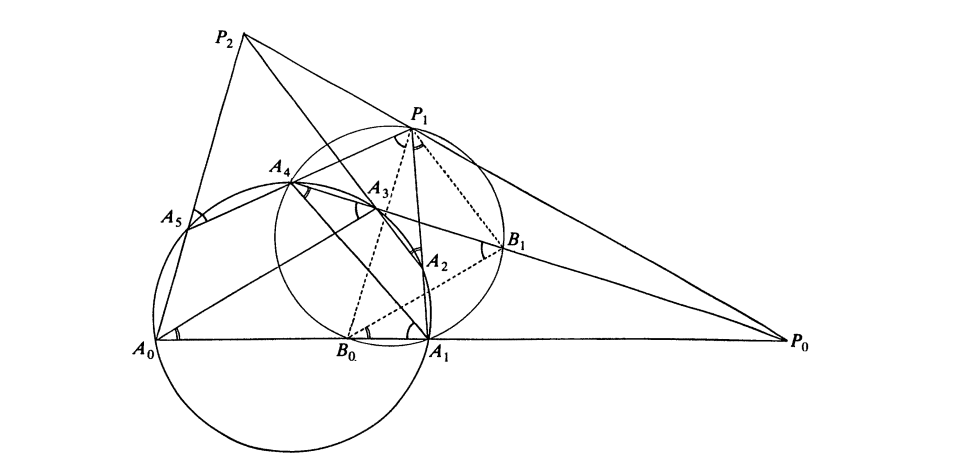
\includegraphics[width=\linewidth]{pascal.png}
   \caption{Figure from \cite{yzeren}.}
  \end{figure}
\end{proof}

\begin{remark}
  Proof adapted from \cite{yzeren}.
\end{remark}

\section{Group Laws on Elliptic Curves}

\begin{definition}
  An elliptic curve is a non-empty, non-singular, degree 3 projective curve. \cite{spallone}
\end{definition}
